\documentclass[11pt,twoside]{article}
\usepackage{geometry}
\usepackage{enumerate}
\usepackage{latexsym,booktabs}
\usepackage{amsmath,amssymb}
\usepackage{graphicx}
\usepackage[singlespacing]{setspace}

\usepackage[backend=bibtex]{biblatex}
\addbibresource{literature.bib}

\geometry{a4paper,left=2cm,right=2.0cm, top=2cm, bottom=2.0cm}

\newtheorem{Definition}{Definition}
\newtheorem{Theorem}{Theorem}
\newtheorem{Lemma}{Lemma}
\newtheorem{Corollary}{Corollary}
\newtheorem{Proposition}{Proposition}
\newtheorem{Algorithm}{Algorithm}
\numberwithin{Theorem}{section}
\numberwithin{Definition}{section}
\numberwithin{Lemma}{section}
\numberwithin{Algorithm}{section}
\numberwithin{equation}{section}


\begin{document}

\pagestyle{empty}

% =============================================================================
% Title page
% =============================================================================
\begin{titlepage}
\vspace*{.5em}
\center
\textbf{\large{The School of Mathematics}} \\
\vspace*{1em}
\begin{figure}[!h]
\centering

\includegraphics[width=180pt]{images/CentredLogoCMYK.jpg}
\end{figure}
\vspace{2em}
\textbf{\Huge{Robust Optimisation Monte Carlo for Likelihood-Free Inference}}\\[2em]
\textbf{\LARGE{by}}\\
\vspace{2em}
\textbf{\LARGE{Vasileios Gkolemis}}\\
\vspace{6.5em}
\Large{Dissertation Presented for the Degree of\\
MSc in Operational Research with Data Science}\\
\vspace{6.5em}
\Large{August 2020}\\
\vspace{3em}
\Large{Supervised by\\Dr. Michael Gutmann}
\vfill
\end{titlepage}

\cleardoublepage

% =============================================================================
% Abstract, acknowledgments, and own work declaration
% =============================================================================
\begin{center}
\Large{Abstract}
\end{center}

Here comes your abstract ...

\clearpage

\begin{center}
\Large{Acknowledgments}
\end{center}

Here come your acknowledgments ...

\clearpage

\begin{center}
\Large{Own Work Declaration}
\end{center}

Here comes your own work declaration

\cleardoublepage



% =============================================================================
% Table of contents, tables, and pictures (if applicable)
% =============================================================================
\pagestyle{plain}
\setcounter{page}{1}
\pagenumbering{Roman}

\tableofcontents
\clearpage
\listoftables
\listoffigures
\cleardoublepage

\pagenumbering{arabic}
\setcounter{page}{1}

\nocite{*}
% \bibliographystyle{abbrv}
\clearpage

\section{Introduction}
\label{sec:introduction}

\subsection{Motivation}

\subsubsection*{\textit{Explanation of Simulation-Based Models}}

A Simulator-Based model is a parameterized stochastic data generating mechanism \cite{Gutmann2016}. The key characteristic is that although we are able to sample (simulate) data points, we cannot evaluate the likelihood of a specific set of observations $y_0$. Formally, a simulator-based model is described as a parameterized family of probability density functions $\{p_{y|\theta}(y)\}_\theta$, whose closed-form is either unknown or intractable to evaluate. Although, evaluating $p_{y|\theta}(y)$ is intractable, sampling is feasible and frequently without huge computational cost. Practically, if we set as $V$ the vector containing the (unobserved) random state of the process, then as a mapping $M(\theta, V) \rightarrow y$

The level of modelling freedom make implicit models particularly captivating; any physical process that can be conceptualized as a computer program of finite (determinstic or stochastic) steps, can be modelled as a Simulator-Based model without any mathematical compromise. This includes any amount of hidden (unobserved) internal variables. On the other hand, this level of freedom comes at a cost; performing inference is particularly demanding from a compuational and mathematical perspective. This constraints the dimensionality of $\theta \in \mathbb{R}^D$ to quite low levels (i.e. $D<20$).

\subsubsection*{\textit{Example}}

For underlying the importance of Simulator-Based models, lets use as example the tuberculosis disease spread model as described in \cite{Tanaka2006}. At each stage we can observe the following events; (a) the transmission of a specific haplotype to a new host (b) the mutation to a different haplotype (c) the exclusion of an infectius host (recovers/dies). The random process, which stops when $m$ infectius hosts are reached, can be parameterized; (a) the transmission rate $\alpha$ (b) the mutation rate $\tau$ and (c) the exclusion rate $\delta$. The outcome of the process is a variable-sized tuple $y_\theta$, containg the size of all different infection groups, as described in figure \ref{fig:tuberculosis_model}. Computing $p(y=y_0|\theta)$ requires tracking all tree-paths that generate the specific tuple along with their probabilities and summing over them. Computing this probability becomes intractable when $m$ grows larger as in real-case scenarios. On the other hand, modeling the data-generation process at a computer program is simple and computationally cheap.

\begin{figure}[!ht]
    \begin{center}
      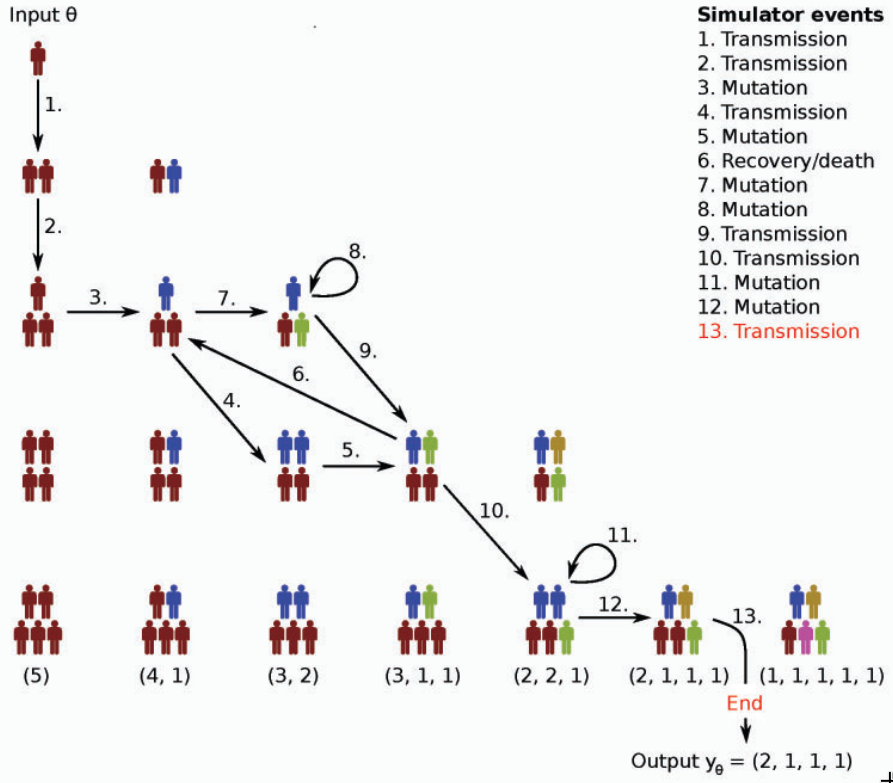
\includegraphics[width=0.49\textwidth]{./images/chapter1/tuber_model_1.png}
      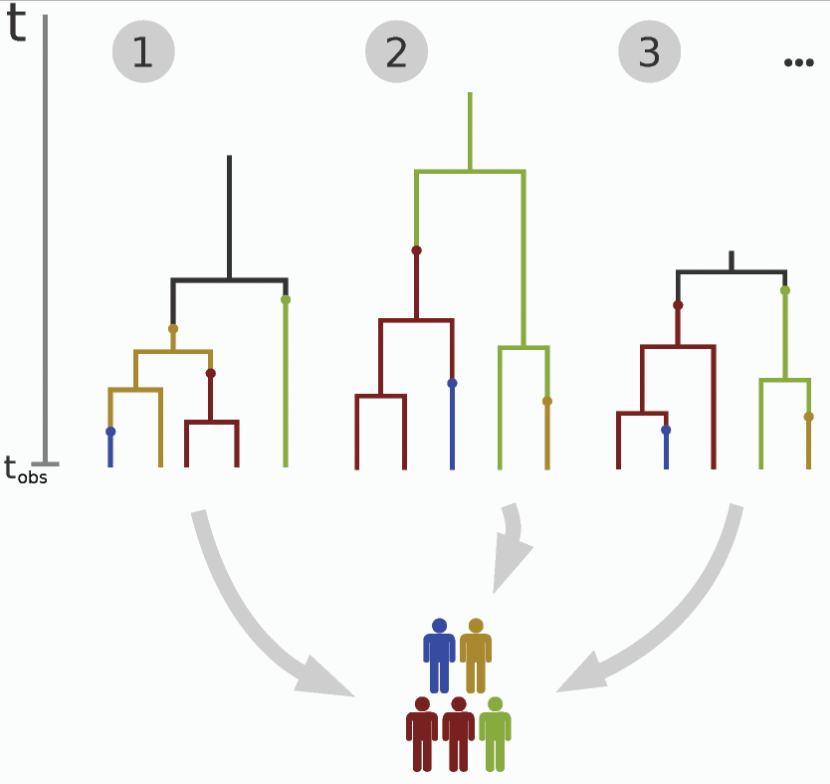
\includegraphics[width=0.42\textwidth]{./images/chapter1/tuber_model_2.png}
    \end{center}
    \caption{Image taken from \cite{Lintusaari2017}}
    \label{fig:tuberculosis_model}
\end{figure}

\subsubsection*{\textit{Goal of Simulation-Based Models}}

As in all Machine Learning (ML) set-ups, the fundamental goal is the derivation of the parameter configuration $\theta^*$ that \textit{describes} well the data (i.e. generates samples $M(\theta^*, V)$ that are as close as possible to the observed data $y_0$). Since Simulation-Based models belong to the broad category of Bayesian Machine Learning, the ultimate goal is to \textit{infer} a posterior distribution $p(\theta|y_0)$ over of all possible configuration set-ups or/and get some samples $\theta \sim p(\theta|y_0)$.

\subsubsection*{\textit{Robust Optimisation Monte Carlo (ROMC) method}}

The ROMC method \cite{Ikonomov2019} is very recent Likelihood-Free approach; its fundamental idea is the transformation of the stochastic data generation process $M(\theta, V)$ to a deterministic function $g(\theta)$, by sampling the variables that the randomness $V_i \sim p(V)$. Hence, we can state that $g(\theta) = M(\theta, V=V_i)$. The ROMC method continues the research line introduced by Meeds et. al \cite{Meeds2015}, by improving some fundamental failure-mode of OMC. ROMC describes a methodology for approximating the posterior through defining and solving deterministic optimisation problems, without enforcing the underlying algorithms for each step; in this sense it can be thought as a meta-algorithm.

\subsubsection*{\textit{Implementation}}

The most important contribution of this work is the implementation of the ROMC method in the Python package Engine for Likelihood-Free Inference (ELFI) \cite{1708.00707}. Since it is very recently published work the ROMC method was not implemented by now in any ML software. This works attempts to provide to the research community a tested and robust implementation for further experimentation.

\subsection{Outline of Thesis}

The remainder of the dissertation is organized as follows. In Chapter 2 we establish the mathematical formulation; more specifically we initially describe the Simulator-Based models and we provide some fundamental algorithms that have been proposed for performing statistical inference. Afterwards, we provide the mathematical description of the ROMC approach \cite{Ikonomov2019}. In Chapter 3, we deal with the implementation part; we initially provide some information regarding the Python package Engine for Likelihood-Free Inference (ELFI) \cite{1708.00707} and subsequently we analyze the implementation details of ROMC in this package. In Chapter 4, we present the functionalities of the ROMC implementation at some real-world examples; this chapter wishes to illustrate the success of the ROMC method and of our implementation at Likelihood-Free tasks. Finally, in chapter 5, we conclude with some thoughts on the work we have done and some future research ideas.

\subsection{Notation}

In this section, we keep an overview of the symbols used throughout the document along with their explanation. We try to keep the notation as consistent as possible, at least to the most central quantities.

\clearpage

\section{Background}
\label{sec:background}

\subsection{Simulator-Based (Implicit) Models}

As already stated, in Simulator-Based models it is impossible to evaluate the quantity $p_{y|\theta}(y)$. The only tool we own is a black-box simulator $M(\theta, V)$ that can be used to generate data. If we denote as $Y_\theta$ the random variable that describes the simulator, then

\begin{equation}
  \int_{y \in B_\epsilon(y_0)} p(y|\theta)dy =  Pr(Y_\theta \in B_\epsilon(y_o)) = Pr(M(\theta, V) \in B_\epsilon(y_o))
  \end{equation}

  On the other hand, the likelihood function can be defined as:
\begin{equation}
  L(\theta) =  \lim_{\epsilon \to 0} c_\epsilon Pr(Y_\theta \in B_\epsilon(y_0)) = \lim_{\epsilon \to 0} c_\epsilon \int_{y \in B_\epsilon(y_0)} p(y|\theta)dy
\end{equation}

and the posterior distribution as:
\begin{equation}
p(\theta|y_0) \propto L(\theta)p(\theta)
\end{equation}

Since $p_{y|\theta}$ cannot be evaluated, so does $L(\theta)$ and subsequently $p(\theta|y_0)$.

\subsubsection{Approximate Bayesian Computation (ABC) Rejection Sampling}

ABC Rejection Sampling is a modified version of Rejection Sampling, for cases when likelihood evaluation is intractable. In the Rejection  method a sample is obtained from the prior $\theta \sim p(\theta)$ and it is maintained with probability $L(\theta)/\text{max}_\theta L(\theta)$. The samples $\theta_i$ obtained with this procedure follow the posterior distribution $p(\theta|y_0)$. Although we cannot use this approach out of the box (evaluating $L(\theta)$ is impossible in our case), we can adjust it with some slight modifications.

In the discrete case scenario where $Y_\theta$ can take a finite set of numbers, the likelihood becomes $L(\theta) = Pr(Y_\theta=y_0)$ and the posterior $p(\theta|y_o) \propto Pr(Y_\theta=y_o)p(\theta)$. Hence, we can sample from the prior $\theta_i \sim p(\theta)$, run the simulator $y_i = M(\theta_i, V)$ and maintain $\theta_i$ if only $y_i = y_0$.

The above method becomes less usefull as the finite set of possible $Y_\theta$ values grows large. As the set grows larger, the probability to maintain a sample becomes smaller. In the limit where the set becomes infinite (i.e. continuous case) the probability becomes zero. In order for the method to work in this set-up, a relaxation is introduced; we relax the acceptance criterion by letting $Y_\theta$ lie in a contiguous area around $y_0$, i.e. $Y_\theta \in B_\epsilon(y_0), \epsilon > 0$. The area can be defined as $B_\epsilon(y_0) := \{y: d(y, y_0) < \epsilon \}$ where $d(\cdot, \cdot)$ can represent any valid distance. With this modification, the maintained samples follow an approximate posterior $p_{d,\epsilon}(\theta|y_0) \propto Pr(Y_\theta \in B_\epsilon(y_0))p(\theta)$, where $B_\epsilon$ is defined by $d, \epsilon$. This procedure is called Rejection ABC algorithm and forms the basis of Likelihood-Free methods.

\subsubsection{Summary Statistics}

When the dimensionality of $Y_\theta \in \mathbb{R}^D$ is high, generating samples inside $B_\epsilon(y_0)$ becomes rare; this is the curse of dimensionality. As an representative example if $B_\epsilon(y_0) := \{ y: ||y - y_0||_2^2 < \epsilon^2 \}$ is a hyper-sphere with radius $\epsilon$ and the prior distribution $p(\theta)$ is a uniform distribution in a hyper-cube with side of length $2/epsilon$, the probability of drawing a sample inside the hyper-sphere becomes:

\begin{equation}
  Pr(Y_\theta \in B_\epsilon(y_0)) = Pr(\theta \in B_\epsilon(y_0)) = \frac{V_{hypersphere}}{V_{hypercube}} = \frac{\pi^{D/2}}{D2^{D-1}\Gamma(D/2)} \rightarrow 0 \text{as} D \rightarrow \infty
\end{equation}

We observe that the probality tends to $0$, independently of $\epsilon$; enlarging $\epsilon$ will not increase the acceptance rate. This produces the need for a mapping $T: \mathbb{R}^{D_1} \rightarrow \mathbb{R}^{D_2}$ where $D_1 > D_2$, redefining the area as $B_\epsilon(y_0) := \{y: d(T(y), T(y_0)) < \epsilon \}$. This process is called measuring the distance at the \textit{summary statistics} level.

\subsubsection{Approximation}

Approximating the posterior as $p(\theta|y_0) \approx p_{d,\epsilon}(\theta|y_0) \propto Pr(Y_\theta \in B_\epsilon(y_0))p(\theta)$ where $B_\epsilon(y_0) := \{y: d(T(y), T(y_0)) < \epsilon \}$ introduces two approximation errors:

\begin{itemize}
\item $\epsilon$ is chosen to be large enough for enough samples to be accepted
  \item Summary Statistics (a) make the distance not a metric in a formal sense, i.e. $d = 0$, even if $y \neq y_0$ (b) make possible disjoint sets of $y$ to lie inside $B_\epsilon{y_0}$
  \end{itemize}

\subsubsection{Optimization Monte Carlo (OMC)}

Optimiza

\subsection{Robust Optimistation Monte Carlo (ROMC) approach}
\label{sec:Techniques}

\subsubsection{Define deterministic optimisation problems}

\subsubsection{Gradient-Based Approach}

\subsubsection{Gaussian Process Approach}

\subsubsection{Weighted Sampling}

\subsection{Engine for Likelihood-Free Inference (ELFI) Package}
\clearpage


\section{Implementation}

\subsection{General Design}

\subsection{Training}

\subsection{Performing the Infernce}

\subsection{Utilities}

\subsection{Computational Complexity}

\clearpage
\section{Experiments}
Add experiments ...

\subsection{Another Example}

\subsection{Execution Time Experiments}

\section{Conclusions}

\subsection{Outcomes}

\subsection{Future Research Directions}
\clearpage

\printbibliography
\clearpage

\appendix
\section*{Appendices}
\addcontentsline{toc}{section}{Appendices}

\clearpage
\section{An Appendix}
\label{app:one}

Some stuff.
\clearpage

\section{Another Appendix}
\label{app:two}

Some other stuff.



\end{document}
